\documentclass{article}

%使用章节标题生产PDF标签
\usepackage[colorlinks=true,linkcolor=blue,urlcolor=blue,citecolor=black]{hyperref}

%中文支持
\usepackage[UTF8]{ctex}
\usepackage{amsmath}
\usepackage{graphicx}
%设置行间距离
\usepackage{Style/setspace}

%设置表格-Align numbers at decimal point
\usepackage{Style/siunitx}

%脚注 --还没调试清楚。
%\usepackage[backend=bibtex,style=verbose-trad2]{Style/biblatex}
\sisetup{
  round-mode          = places, % Rounds numbers
  round-precision     = 2, % to 2 places
}

%设置目录显示深度
%\setcounter{tocdepth}{2} % Show sections
%\setcounter{tocdepth}{2} % + subsections
%\setcounter{tocdepth}{3} % + subsubsections
%\setcounter{tocdepth}{4} % + paragraphs
%\setcounter{tocdepth}{5} % + subparagraphs

%用于设置多表格
\usepackage{Style/multirow/multirow} % Required for multirows

%代码
\usepackage{Style/listings/listings}
\usepackage{Style/color}

\renewcommand\lstlistingname{C++} % Change language of section name

\lstset{ % General setup for the package
	language=C++,
	basicstyle=\small\sffamily,
	numbers=left,
 	numberstyle=\tiny,
	frame=tb,
	tabsize=4,
	columns=fixed,
	showstringspaces=false,
	showtabs=false,
	keepspaces,
	commentstyle=\color{red},
	keywordstyle=\color{blue}
}

%超链接
\usepackage{hyperref}


\usepackage{Style/enumitem}


\title{Latex学习教程}
\date{2018-03-03}
\author{zuisixian}




\begin{document}
%we don't want to have that page number showing up there,remove it
\pagenumbering{gobble} 
\maketitle
%设置double行间距
\doublespacing

\tableofcontents
%恢复
\doublespacing

\newpage
%hanging it back on the next page numbers
\pagenumbering{arabic}


  \section{环境搭建}
  %用于在本section中设置目录的显示深度
  %\addtocontents{toc}{\setcounter{tocdepth}{1}} % Set depth to 1
  下载latex编译器MikTex/CTEX/TEXLive都可以,编译器的话可以选择TexMaker,TexStudio,
  或者就是普通的编辑器如atom、VSCode。
    \subsection{下载MikTex,TexMaker}

    %\newpage
    \subsection{vscode设置}
    在左下角有个设置按钮,点击进入设置,可以对工作区或者用户层面进行设置,按照图 \ref{fig:set1}进行设置。
    \begin{figure}
      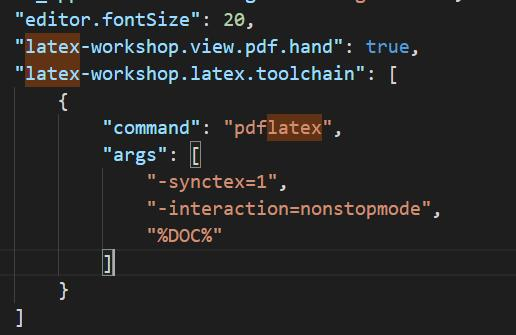
\includegraphics[width=\linewidth]{image/vscode-setting.jpg}
      \caption{设置界面.}
      \label{fig:set1}
    \end{figure}

    这是一个段落
    \begin{lstlisting}
    #!/usr/bin/perl
    print S(@ARGV);sub S{$r=(@_[0]%4==0&&@_[0]%100!=0)||@_[0]%400=0;}
    int main(){
      cout<<"Hello world"<<endl;
      return 0;
    }
    \end{lstlisting}

    This is my link: \href{http://github.com/zuisixian/}{zuisixian}.
    \url{http://github.com/zuisixian}
    \begin{itemize}
      \item[--] One
      \item[--] Two
      \item Three
    \end{itemize}

    \begin{enumerate}
      \item One
      \item Two
      \item Three
    \end{enumerate}

    \begin{enumerate}
      \item One
        \begin{enumerate}
          \item Two
            \item Three
            \item Four
        \end{enumerate}
        \item Five
        \item Six
    \end{enumerate}
    
    \begin{enumerate}[label=(\roman*)]
      \item xxxxx

    \end{enumerate}


    \paragraph{}
      这是一个段落

    





  \section{Latex基础}
  语法
  \begin{equation}
    f(x) = x^2
  \end{equation}

  \begin{figure}
    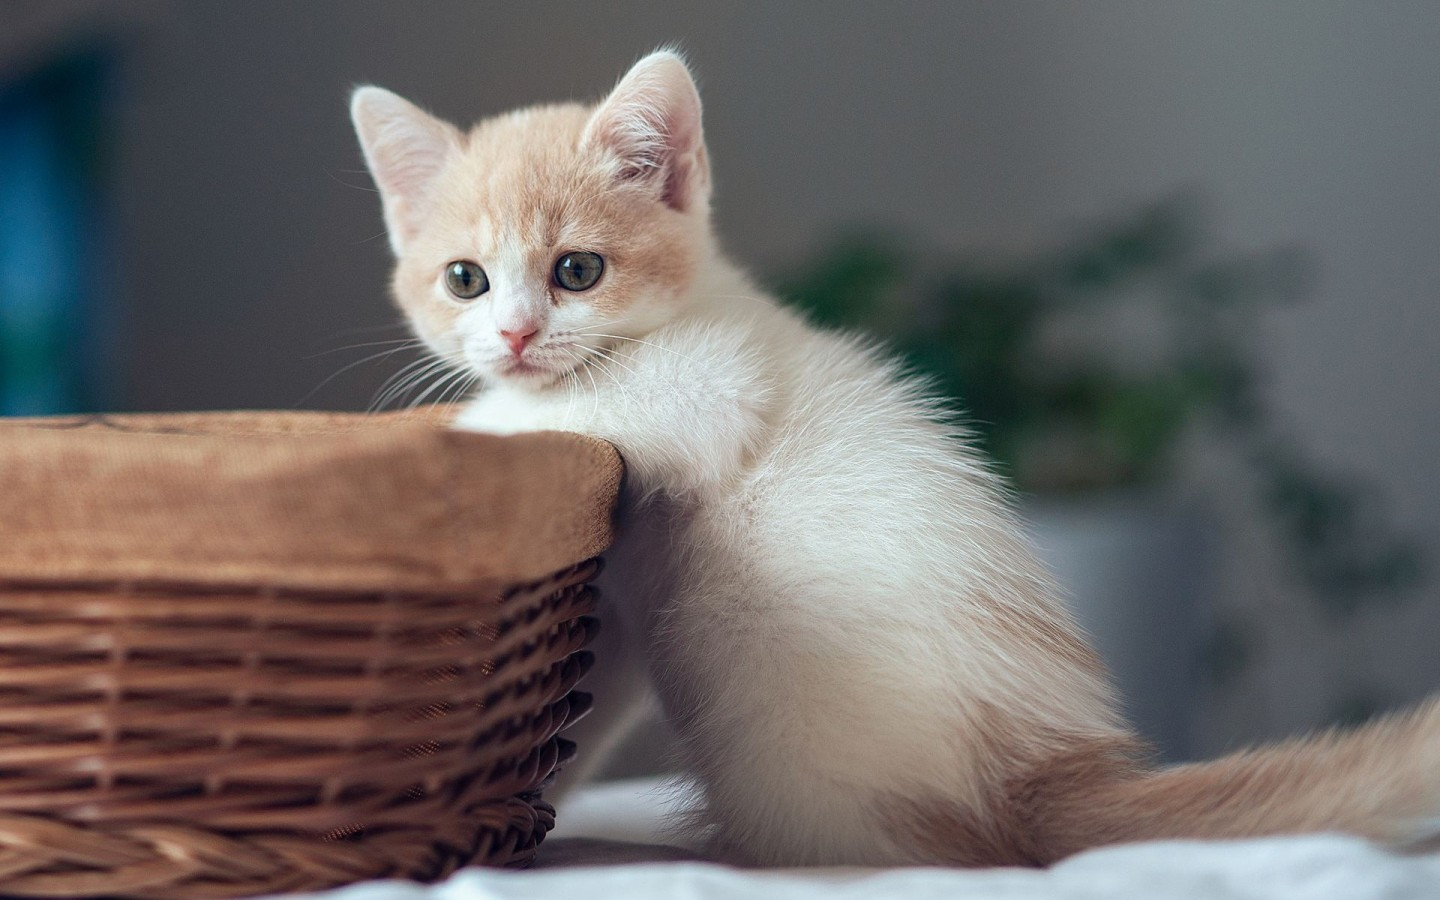
\includegraphics[width=\linewidth]{image/qwe.jpg}
    \caption{A CAT.}
    \label{fig:cat1}
  \end{figure}
  这是一个表格:
  \begin{table}[h!]
    \begin{center}
      \caption{我的第一个表格.}
      \label{tab:table1}
      \begin{tabular}{|l|S|r|r} % <-- Alignments: 1st column left, 2nd middle and 3rd right, with vertical lines in between
        \textbf{Value 1} & \textbf{Value 2} & \textbf{Value 3}& \textbf{Value 4}\\
        $\alpha$ & $\beta$ & $\gamma$ & $\Delta$ \\
        \hline
        \multirow{2}{*}{12} & 1110.1 & a& 2\\ % <-- Combining 2 rows with arbitrary with (*) and content 12
        & 10.1 & b\\ % <-- Content of first column omitted.
        \hline
        1 & 1110.1 & a & 1\\
        \hline 
        \multicolumn{2}{|c|}{12} & a\\ % <-- Combining two cells with alignment c| and content 12.
        \hline
        \multicolumn{2}{|c|}{\multirow{2}{*}{1234}} & a\\ % <-- Multicolumn spanning 2 columns, content multirow spanning two rows
        \multicolumn{2}{|c|}{} & b\\ % <-- Multicolumn spanning 2 columns with empty content as placeholder
        \hline
        2 & 10.1 & b & 2\\
        3 & 23.113231 & c&3\\
        4 & 23.23443 & d & 4\\
      \end{tabular}
    \end{center}
  \end{table}



  
  图 \ref{fig:cat1} shows a cat.

  Random citation \cite{melissa:1} embeddeed in text.


  \section{LaTeX.sty文件缺失解决办法}
  从CTAN的网站上下载pkg,解压后有pkg.ins和pkg.dtx,
  在终端执行pdflatex pkg.ins会生成pkg.sty,
  也可以拷贝到系统目录,也可以放到用户文件所在路径,我是放在root/Sytle中

  如果编译时缺失pkg,可以查看编译的时候打出的log,
  很多包的查找路径都有输出在log里面。

  
  \href{https://www.ctan.org/pkg}{pkg下载地址}
  或者\href{http://mirrors.cqu.edu.cn/CTAN/macros/latex/contrib/}{pkg下载地址2}

  生产帮助文档:
  latex pkg.dtx会生成pkg.dvi的文件,再dvips pkg.dvi即可生成帮助文档。

  pkg放入路径:C:/CTEX/MiKTeX/tex/latex/
  在这个路径下建立一个文件夹,譬如pkgname,
  然后把pkg.sty放到这里,接着在你的电脑里找到MikTex的settings这个程序,
  settings有两个,选择后面括号里有admin的那个,打开以后
  在general选项卡下有Refresh FNDB按钮,
  点击,过一会,这个package就会加入MikTex的路径中,
  然后在你的tex文件中就可以使用这个package了

  按照图 \ref{fig:set2}进行设置。
  \begin{figure}
    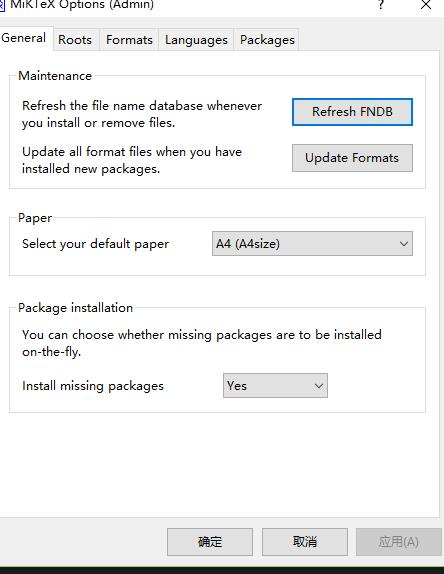
\includegraphics[width=\linewidth]{image/miktex-setting.jpg}
    \caption{设置界面.}
    \label{fig:set2}
  \end{figure}


  Latex错误:The remote package repository is not registered. You have to choose another repository. 
  解决办法: 
  (1)MikTex Package manager => Repository => Change Package Repository => Package shall be installed from the Internet => 下一步 => 完成,这样就连接上网络了。 
  (2)然后再MikTex Package manager => Repository => Synchronize 就完成同步了。 
  (3)然后再找到需要安装的宏包,选中,+号,即可。 



  \bibliography{first} 
  \bibliographystyle{ieeetr}




  \begin{appendix}
    \listoffigures
    \listoftables
  \end{appendix}




\end{document}
